\documentclass{article}

% The provided Overleaf project contains neurips.sty. When the style file is
% present, this document uses the required formal NeurIPS layout. The fallback
% settings below keep this file compilable when previewed outside Overleaf.
\IfFileExists{neurips.sty}{
  \usepackage[final,nonatbib]{neurips}
}{
  \usepackage[margin=0.72in]{geometry}
}

\usepackage[utf8]{inputenc}
\usepackage[T1]{fontenc}
\usepackage{amsmath,amssymb}
\usepackage{booktabs}
\usepackage{array}
\usepackage{graphicx}
\usepackage{microtype}
\usepackage{xcolor}
\usepackage{url}
\usepackage{hyperref}
\usepackage{subcaption}

\title{Efficient Ink-Wash Generation with PixArt-Sigma LoRA and 20-to-4-to-2 Step Distillation}

% TODO: Replace the placeholders below with the final names and student IDs.
\author{
Group 19\\[4pt]
\small
Yulong Sheng (1011838843)
\quad
Housen Zhu (1008117477)
\quad
Poon Chun Kit (1011866893)
}

\date{}

\begin{document}

\pagenumbering{arabic}
\maketitle
\thispagestyle{plain}
\setcounter{page}{1}


\begin{abstract}
We present a parameter-efficient framework for adapting and accelerating
PixArt-$\Sigma$ for Chinese ink-wash image generation. A rank-16 LoRA is first
trained on a curated 209-image subset to learn domain-specific brushwork,
ink diffusion, and negative-space composition. The resulting 20-step Style
Teacher is then compressed through latent-trajectory distillation into four-
and two-step Students. We evaluate prompt alignment, distributional similarity,
and inference latency on 30 held-out prompts with four fixed seeds. The four-step
Student preserves the Teacher's CLIP alignment while providing approximately a
sixfold speedup, whereas the two-step Student retains 96.8\% of the Teacher's
alignment with an approximately 11.8-fold speedup. These results identify four
steps as the quality-oriented operating point and two steps as the
latency-oriented alternative for interactive generation.
\end{abstract}

% TODO (team): Insert the required attestation of teamwork here if the course
% template asks for it. Keep this statement concise.

\section{Introduction}

Large text-to-image diffusion models provide strong general-purpose generation, but adapting them to a small, coherent artistic domain remains difficult. In our setting, the target is expressive Chinese ink-wash imagery characterized by sparse composition, diffused ink, visible brush variation, and selective colour. A general PixArt-$\Sigma$ model can respond to explicit style words, yet its outputs do not consistently reproduce the visual statistics of the curated collection. Full fine-tuning is also impractical for our data and compute budget, while the standard 20-step sampler is too slow for interactive use.

We therefore study a combined \emph{adapt-and-accelerate} pipeline. First, Low-Rank Adaptation (LoRA) specializes a frozen PixArt-$\Sigma$ transformer using paired ink-wash images and captions. Second, the selected 20-step adapter acts as a Teacher whose denoising trajectories supervise progressively faster Students. Our final route reduces inference from 20 transformer evaluations to four and then two. The objective is not only lower latency: the accelerated model must preserve prompt semantics, the learned ink-wash domain, and recognizable object structure. This separation also supports controlled evaluation: Teacher checkpoints are selected on held-out prompts, while Students are compared against the fixed Teacher at matched seeds and conditioning.

\section{Preliminaries and Problem Formulation}

\paragraph{Latent diffusion.}
Let $E$ and $D$ be the frozen VAE encoder and decoder, and let $z_0=E(x)$ denote the clean image latent. For diffusion time $t$, training constructs
\begin{equation}
z_t=\sqrt{\bar{\alpha}_t}\,z_0+\sqrt{1-\bar{\alpha}_t}\,\epsilon,
\qquad \epsilon\sim\mathcal{N}(0,I),
\end{equation}
and a text-conditioned PixArt transformer predicts the denoising target from $(z_t,t,c)$, where $c$ is the frozen T5 caption embedding. Generation starts from Gaussian noise and repeatedly applies the transformer and scheduler before decoding the final latent with $D$ \cite{chen2024pixartsigma,song2021ddim}.

\paragraph{Low-rank adaptation.}
For a frozen linear map $W\in\mathbb{R}^{d_{\mathrm{out}}\times d_{\mathrm{in}}}$, LoRA learns
\begin{equation}
W'=W+\frac{\alpha}{r}BA,
\quad A\in\mathbb{R}^{r\times d_{\mathrm{in}}},\quad
B\in\mathbb{R}^{d_{\mathrm{out}}\times r},\quad r\ll \min(d_{\mathrm{in}},d_{\mathrm{out}}).
\end{equation}
Only the low-rank matrices are optimized \cite{hu2022lora}. In our implementation, adapters are attached to attention projections and feed-forward/projection layers; the VAE, T5 encoder, and original PixArt weights remain frozen.

\paragraph{Objective.}
Given a style dataset $\mathcal{D}=\{(x_i,y_i)\}$, we seek a Teacher adapter $\phi_T$ and Student adapter $\phi_S$ that jointly balance style transfer, prompt adherence, structural quality, and computation. Formally, the Student should approximate Teacher transitions on the same latent trajectory while using $K\in\{4,2\}$ transformer calls rather than 20. This is evaluated with held-out prompts, fixed seeds, CLIP-based prompt alignment, distributional image metrics, and visual inspection; no single metric is treated as a complete measure of image quality.

\section{Design}

The system has three reusable layers:
\begin{equation}
\small
\text{images/captions}
\rightarrow \text{VAE and T5 caches}
\rightarrow \text{20-step LoRA Teacher}
\rightarrow \text{4-step Student}
\rightarrow \text{2-step Student}.
\end{equation}
The corpus contains 260 image--caption pairs spanning 209 plants, 30 animals, and 21 other subjects; the primary Teacher and distillation route use the 209-image plant subset. We precompute clean 512-pixel VAE latents and length-300 T5 embeddings once, validate their sample fingerprint and ordering, and reuse them across runs. This removes repeated VAE/T5 memory cost and makes Teacher comparisons reproducible on limited hardware.

The Teacher is the frozen PixArt-$\Sigma$ backbone plus one style LoRA. The Students keep the same backbone and attach trainable low-rank modules to the same target layers, which preserves parameter efficiency and adapter portability. Distillation is performed in latent space: the 4-step Student learns four consecutive five-step Teacher intervals, $(0,5)$, $(5,10)$, $(10,15)$, and $(15,20)$; the 2-step Student learns two ten-step intervals, $(0,10)$ and $(10,20)$. The 4-step adapter initializes the 2-step stage, forming a progressive 20-to-4-to-2 route rather than learning the hardest compression directly \cite{salimans2022progressive}.

\section{Methodology}

\paragraph{Teacher training.}
We encode each caption and image once, then sample a cached clean latent $z_0$, time $t$, and noise $\epsilon$ during training. The noisy latent from Eq.~(1) is passed through PixArt-$\Sigma$ with the LoRA adapter, and the adapter is optimized using mean-squared diffusion loss,
\begin{equation}
\mathcal{L}_{\mathrm{teach}}
=\mathbb{E}_{(z_0,c),t,\epsilon}
\left[\left\|f_{\theta,\phi_T}(z_t,t,c)-\epsilon\right\|_2^2\right].
\end{equation}
The primary run uses rank and alpha 16, batch size one, learning rate $10^{-5}$, and checkpointing every 1,000 optimizer updates. The Teacher is selected from intermediate checkpoints using held-out prompts and visual inspection, instead of assuming that the final checkpoint generalizes best.

\paragraph{Offline trajectory supervision.}
With the selected Teacher frozen, we generate deterministic 20-step latent trajectories for 627 prompt variants and two seeds, producing 1,254 trajectories with 21 stored states each. Every record contains its text conditioning, seed, scheduler timesteps, initial noise, and intermediate latents. This cache allows Student training without holding Teacher and Student models in GPU memory simultaneously.

\paragraph{Student loss and progressive compression.}
Most updates teach a Student to jump between cached phase boundaries. If $z_s^T$ and $z_e^T$ are Teacher states at a phase start and end, the Student prediction $\hat z_e^S$ is trained with pseudo-Huber loss
\begin{equation}
\mathcal{L}_{\mathrm{traj}}
=\sqrt{\|\hat z_e^S-z_e^T\|_2^2+c^2}-c,
\qquad c=10^{-3}.
\end{equation}
To retain the original diffusion field, 20\% of updates instead use the Teacher diffusion target with an MSE anchor loss, while 80\% use trajectory targets. The 4-step stage uses a learning rate of $5\times10^{-6}$. Its adapter then initializes the 2-step stage, which uses $2\times10^{-6}$. For the second phase of the 2-step Student, half of the starting latents are generated by the current Student rather than copied from the Teacher cache; this on-policy correction reduces train--test mismatch caused by errors accumulated after the first jump.

Teacher evaluation uses classifier-free guidance selected during validation. The distilled Students use guidance scale 1.0 and a single conditional branch, so the reported four-step and two-step models require exactly four and two transformer calls. All experiments use the same cached features, scheduler definition, checkpoint metadata, and fixed evaluation seeds to isolate the effects of LoRA adaptation and step reduction \cite{group19repo}.

\section{Numerical Experiments}

\subsection{Protocol and implementation details}
We evaluate two questions: whether a LoRA transfers the Chinese ink-wash domain
beyond exact training captions, and whether the adapted 20-call model can be
compressed to four or two Transformer calls.  Experiments use the coherent
209-plant subset of the 260 validated image--caption pairs at $512\times512$.
The rank-16 Style Teacher uses 20 DPM-Solver++ steps and CFG 1.5.  The primary
rank-16 Students are the 4,500-update 4-step checkpoint and its 7,000-update
2-step successor; both use CFG 1.0 without an unconditional branch.  Full
training and cache settings are deferred to the Appendix.

The held-out benchmark contains 30 unseen prompts and four fixed seeds per
prompt, or 120 images per model.  We report CLIP ViT-B/32 text--image cosine
similarity, unbiased squared CMMD against all 209 real plant images, warmed-up
median latency, and exact forward-call count.  Each seed position forms one
30-prompt replicate; Table~\ref{tab:primary} reports mean $\pm$ sample SD over
four replicates.  No additional training was performed for these analyses.
CMMD is the unbiased squared MMD between normalized CLIP image features, using
a Gaussian RBF kernel of bandwidth 10 and all 209 real plant images as the
reference distribution.  The same prompts and seed positions are retained for
every model, and latency is recorded after warm-up in one software/hardware
environment so that only the adapter and call count change.

\subsection{Style adaptation and held-out generation}
We compared ranks 4, 8, 16, and 32 every 1,000 updates to 10,000 under matched
20-step sampling.  The best rewritten-palm result improves CLIP from 0.3399 to
0.3561 (+4.7\%), while an unseen misty-mountain prompt improves from 0.3615 to
0.3720 (+2.9\%).  Because later checkpoints often decline and the best rank is
prompt-dependent, held-out selection is more reliable than training longer.

For the preferred unseen fishing-boat prompt at seed 10163
(Figure~\ref{fig:fourway}), Teacher B replaces the base model's photographic
appearance with monochrome brushwork and negative space.  Both Students preserve
the composition, although the 2-step output is softer.

\begin{figure}[t]
  \centering
  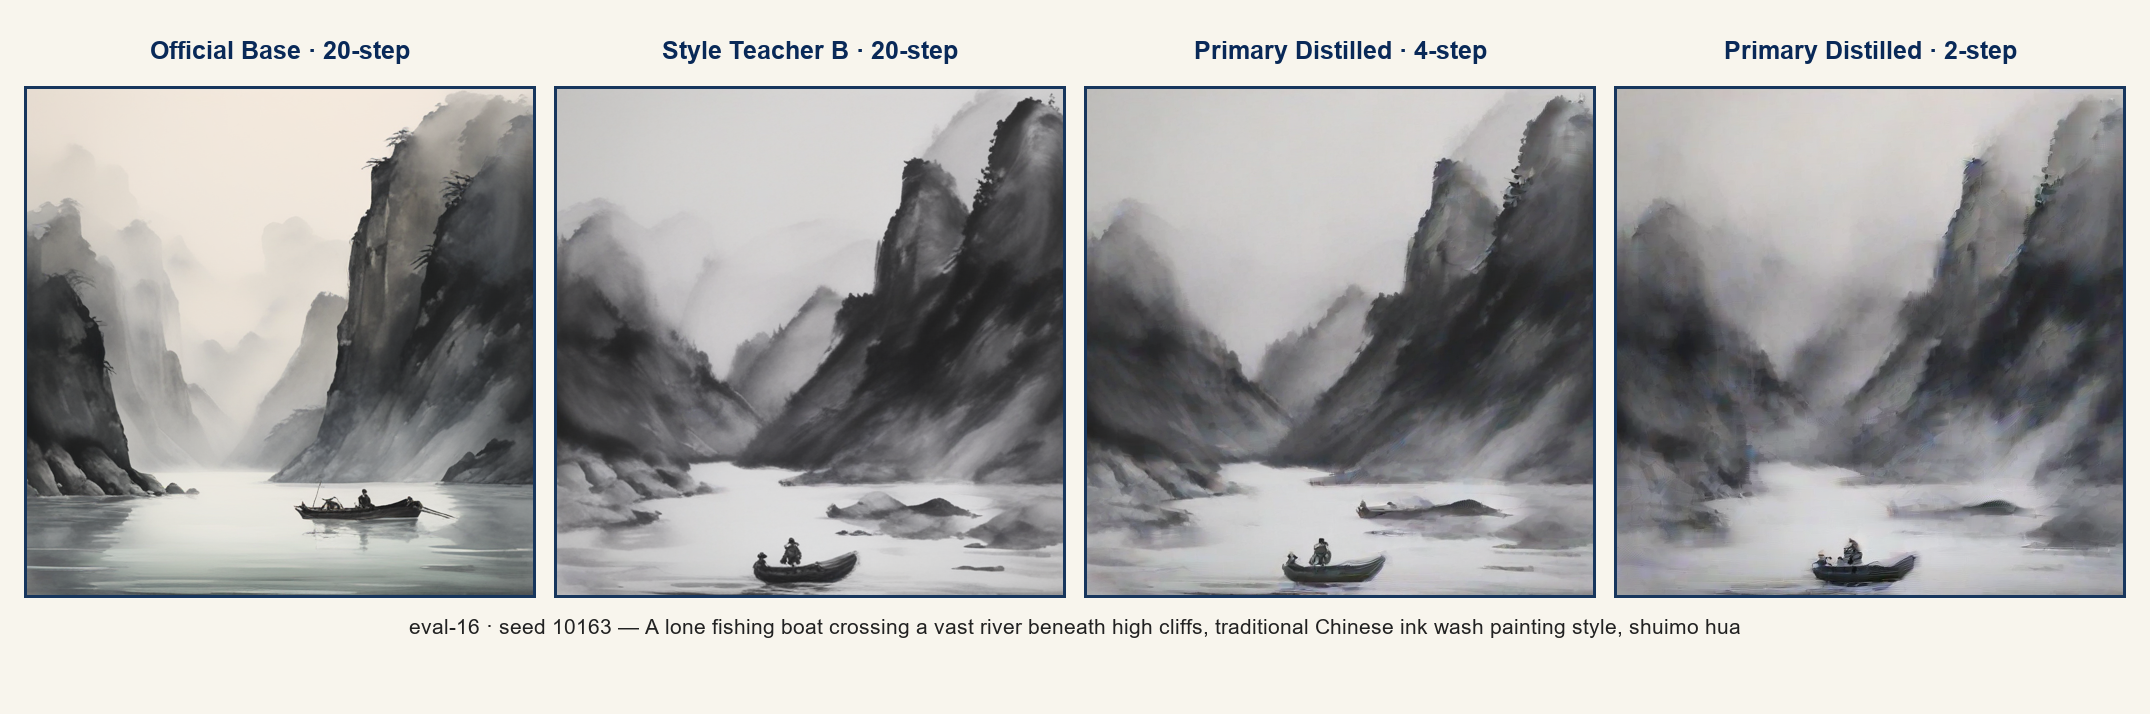
\includegraphics[width=0.92\linewidth]{figures/eval16_fourway.png}
  \caption{Same unseen prompt and seed for the official 20-step base, 20-step
  Style Teacher B, primary 4-step student, and primary 2-step student.}
  \label{fig:fourway}
\end{figure}

\subsection{Few-step quality, efficiency, and seed variance}
The 4-step Student preserves 100.65\% of Teacher CLIP at 5.99$\times$ speedup;
the 2-step Student retains 96.84\% at 11.78$\times$ speedup.  Its CMMD lies only
2.00\% below the predefined $1.5\times$-Teacher limit, making four steps the
quality-oriented point and two steps the latency-oriented alternative.

\begin{table}[t]
  \caption{Held-out mean $\pm$ SD over four 30-prompt seed replicates.}
  \label{tab:primary}
  \centering
  \small
  \setlength{\tabcolsep}{3.8pt}
  \begin{tabular}{lrrrrr}
    \toprule
    Model & Calls & CLIP $\uparrow$ & CMMD $\downarrow$ & Time (s) $\downarrow$ & Speedup \\
    \midrule
    Teacher B & 20 & $0.3651\!\pm\!0.0040$ & $0.000947\!\pm\!0.000056$ & $2.871\!\pm\!0.006$ & 1.00$\times$ \\
    4-step & 4 & $\mathbf{0.3674\!\pm\!0.0049}$ & $0.001070\!\pm\!0.000047$ & $0.484\!\pm\!0.009$ & 5.99$\times$ \\
    2-step & 2 & $0.3535\!\pm\!0.0025$ & $0.001385\!\pm\!0.000102$ & $\mathbf{0.243\!\pm\!0.010}$ & \textbf{11.78$\times$} \\
    \bottomrule
  \end{tabular}
\end{table}

The 4-step CLIP advantage (0.0024) is smaller than replicate SD and therefore
indicates preservation, not a significant gain.  Within-prompt seed variation
is larger still (Appendix), so single-seed comparisons are unreliable.
Specifically, the root-mean-square within-prompt seed SD is 0.0230, 0.0200, and
0.0213 for Teacher, 4-step, and 2-step respectively.  The 2-step CMMD also has
the largest replicate SD ($1.02\times10^{-4}$), reinforcing its role as the
latency-oriented rather than fidelity-equivalent operating point.

\subsection{What happens between the reported endpoints?}
Inference-only evaluation on \texttt{eval-16} (four seeds) decodes every latent
state.  Figure~\ref{fig:intermediate} shows that Teacher CLIP stays near 0.12
through call 14 before reaching $0.346\pm0.049$ at call 20.  The 4-step scores
are 0.125, 0.122, 0.130, and $0.368\pm0.020$; the 2-step scores are 0.122 and
$0.366\pm0.014$.  Most visible alignment emerges in the final learned jump.
Decoded states appear in the Appendix; early noisy $x_t$ makes per-call CLIP a
diagnostic rather than a training objective.
The Teacher curve begins its measurable rise only at calls 17--18 (CLIP 0.174
and 0.234), whereas each Student concentrates this transition into its final
call.  This behavior confirms that few-step inference learns large trajectory
jumps rather than merely terminating the original 20-step solver early.

\begin{center}
  \centering
  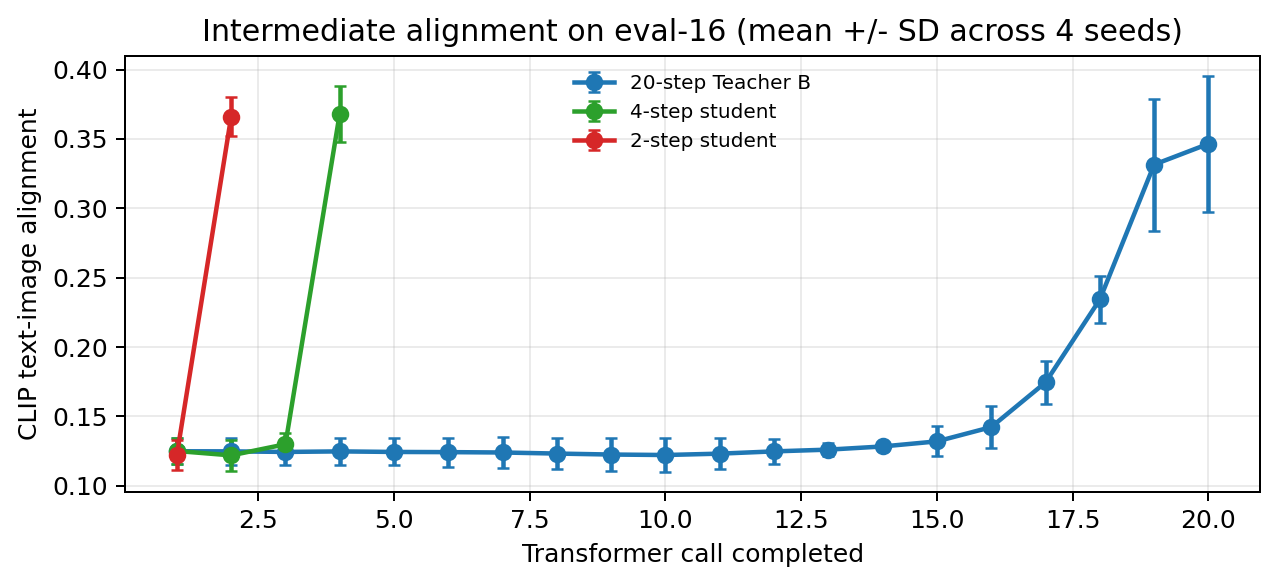
\includegraphics[width=0.62\linewidth]{figures/eval16_intermediate_clip_curve.png}
  \captionof{figure}{CLIP mean $\pm$ SD over four seeds after every call for the
  same unseen prompt.  The Appendix shows the decoded intermediate states.}
  \label{fig:intermediate}
\end{center}
\par\medskip


\section{Discussion}

\subsection{Answers to core research questions}

\textbf{RQ1: Domain adaptation and generalization under low-rank fine-tuning.}
\textit{Does low-rank adaptation on a small curated dataset transfer Chinese ink-wash style without overfitting?} \\
Rank-16 LoRA (13.8\,M parameters, $\sim$0.40\% of the backbone) successfully adapts PixArt-Sigma to the Chinese ink-wash aesthetic (\textit{shuimo hua}), capturing monochrome brushwork, wet-ink diffusion on \textit{xuan} paper, and negative space (\textit{liubai}). Generalization on unseen prompts peaks early ($\sim$step 4,000) before overfitting to training captions. Dataset purity proves decisive: 209 clean plant images (\texttt{plant209}, CMMD 0.001229) clearly outperform 260 images mixed with photographic noise (\texttt{n260}, CMMD 0.001445), demonstrating that curation quality matters more than scale.

\textbf{RQ2: Few-step trajectory distillation, guidance elimination, and latency--quality trade-offs.}
\textit{Can a 20-step teacher be compressed into 4-step and 2-step students while preserving quality, and what governs the step-count trade-off?} \\
Yes. Trajectory distillation (80\% trajectory loss + 20\% diffusion anchor) successfully compresses the 20-step teacher into few-step regimes. Training students at $\text{CFG}=1.0$ eliminates the negative guidance pass, halving the required forward passes per step. The 4-step student achieves a $5.99\times$ speedup (0.480\,s vs.\ 2.871\,s) with complete quality retention (100.65\% CLIP alignment at $0.3674 \pm 0.0049$ and low CMMD $0.001070 \pm 0.000047$). Distilling to 8 or 16 steps is unnecessary because visual fidelity already saturates at 4 steps, adding a $2\times\text{--}4\times$ latency penalty without measurable gain. Conversely, pushing distillation to 2 steps unlocks the real-time interactive regime (0.243\,s, $11.78\times$ speedup) with 96.84\% CLIP retention ($0.3535 \pm 0.0025$) and acceptable style distance (CMMD $0.001385 \pm 0.000102$, within the $1.5\times$ teacher limit), establishing 4 steps as the fidelity-oriented benchmark and 2 steps as the speed-oriented deployment point.

\textbf{RQ3: Intermediate-step dynamics, sampling mechanics, and few-step jump distillation.}
\textit{What occurs at each step during 20-step generation, how does training differ from sampling, and how do few-step students compress these dynamics?} \\
\textbf{Sampling steps} and \textbf{training updates} operate under distinct mechanics. During 20-step Teacher sampling, solving the reverse ODE at $\text{CFG}=1.5$ requires 40 forward passes. Decoding intermediate latents $x_t$ shows that visual emergence is non-linear: steps 1--14 ($t \in [999, 300]$) remain off-manifold noise (CLIP $\approx 0.12$), coarse composition emerges at steps 15--17, and fine brushwork with negative space resolves only in the final two steps ($t \le 100$, CLIP $\ge 0.35$). Crucially, Teacher \textbf{training} samples a single random $t$ per update rather than rolling out 20 steps. \textbf{Student distillation} bridges this gap: using offline cached trajectories, 4-step and 2-step students learn direct macroscopic jumps (spanning 5 and 10 teacher steps per call) onto the clean manifold at $\text{CFG}=1.0$, bypassing numerical ODE solver failure.

\subsection{Variance dynamics and evaluation reliability}
Across 30 test prompts, seed variation ($\text{RMS SD} \approx 0.020\text{--}0.023$) exceeds model-level differences. Evaluating 4 fixed seeds across held-out prompts (120 images per model) prevents single-seed bias and confirms that the 4-step student reliably matches teacher performance.

\section{Conclusions}

\subsection{Summary of Contributions and Key Insights}
This work demonstrates an efficient adapt-and-accelerate framework for specialized artistic diffusion synthesis. First, a lightweight rank-16 LoRA adapter (13.76\,M parameters, $\sim$0.40\% of the DiT backbone) trained on a curated 209-image plant corpus reliably captures wet-ink diffusion on \textit{xuan} paper and negative space (\textit{liubai}), showing that dataset purity and early stopping ($\sim$step 4,000) outweigh dataset scale. Second, progressive trajectory distillation ($20 \to 4 \to 2$ steps) combined with classifier-free guidance elimination ($\text{CFG}=1.0$) and 50\% on-policy roll-in establishes an optimal Pareto frontier: the 4-step student provides the quality-oriented regime (0.480\,s, $5.99\times$ speedup, 100.65\% CLIP retention), while the 2-step student unlocks real-time interactive generation (0.243\,s, $11.78\times$ speedup, 96.84\% CLIP retention). Finally, intermediate latent analysis reveals that image emergence in diffusion ODEs is non-linear, and distilled students successfully bypass numerical solver failure at $\le 4$ steps by executing direct learned macroscopic jumps.

\subsection{Limitations and Future Work}
While effective, our evaluation was conducted at $512 \times 512$ on floral/landscape compositions, and the 2-step student exhibits slight softening of dry-brush micro-textures relative to the teacher. Future research will explore single-step consistency distillation and rectified flow for sub-100\,ms generation, adversarial objectives to sharpen ultra-few-step brushwork, and domain-specific quantitative metrics measuring ink bleeding gradients and negative space ratios.


\clearpage
\begin{thebibliography}{9}

\bibitem{chen2024pixartsigma}
J. Chen et al.
\newblock PixArt-$\Sigma$: Weak-to-Strong Training of Diffusion Transformer for 4K Text-to-Image Generation.
\newblock In \emph{European Conference on Computer Vision}, 2024.

\bibitem{hu2022lora}
E. J. Hu et al.
\newblock LoRA: Low-Rank Adaptation of Large Language Models.
\newblock In \emph{International Conference on Learning Representations}, 2022.

\bibitem{song2021ddim}
J. Song, C. Meng, and S. Ermon.
\newblock Denoising Diffusion Implicit Models.
\newblock In \emph{International Conference on Learning Representations}, 2021.

\bibitem{salimans2022progressive}
T. Salimans and J. Ho.
\newblock Progressive Distillation for Fast Sampling of Diffusion Models.
\newblock In \emph{International Conference on Learning Representations}, 2022.

\bibitem{group19repo}
Group 19.
\newblock Efficient PixArt-Sigma LoRA.
\newblock \url{https://github.com/jackyckp/efficient-pixart-sigma-lora/tree/ZHS}, 2026.

\end{thebibliography}


\clearpage
\appendix
\section{Reproducibility and Additional Results}
\label{app:repro}

\subsection{Exact primary-model configuration}
Table~\ref{tab:appendix-config} records implementation details omitted from the
main numerical section for space.  Cached VAE latents are FP16 tensors of shape
$4\times64\times64$ and T5-XXL prompt embeddings have shape $300\times4096$.
The prompt bank contains three variants of each of 209 plant captions and two
deterministic seeds per prompt, producing 1,254 teacher trajectories.

\begin{table}[h]
  \caption{Primary distillation configuration.}
  \label{tab:appendix-config}
  \centering
  \small
  \setlength{\tabcolsep}{4pt}
  \begin{tabular}{>{\raggedright\arraybackslash}p{0.17\linewidth}
                  >{\raggedright\arraybackslash}p{0.34\linewidth}
                  >{\raggedright\arraybackslash}p{0.39\linewidth}}
    \toprule
    Component & Optimization & Inference / phase mapping \\
    \midrule
    Teacher B & Rank/alpha 16/16 style LoRA & 20-step DPM-Solver++, CFG 1.5 \\
    4-step student & LR $5\times10^{-6}$; selected at 4,500/6,000 updates &
      CFG 1.0; trajectory indices $0\!\to\!5\!\to\!10\!\to\!15\!\to\!20$ \\
    2-step student & LR $2\times10^{-6}$; 7,000 updates; 50\% on-policy roll-in &
      CFG 1.0; trajectory indices $0\!\to\!10\!\to\!20$ \\
    Both students & Rank/alpha 16/16; 80\% pseudo-Huber trajectory loss; 20\%
      clean-latent anchor & FP16 base, FP32 LoRA; no unconditional CFG branch \\
    \bottomrule
  \end{tabular}
\end{table}

\subsection{Seed-resolved metrics}
Each column $s_1$--$s_4$ in Table~\ref{tab:seed-resolved} is the mean CLIP score
for the same 30 unseen prompts under one seed position.  The final column instead
computes the root-mean-square of the within-prompt SD across four seeds.  The
4-step aggregate gain is smaller than replicate variation, while all three
models show much larger example-level seed sensitivity.

\begin{table}[h]
  \caption{Seed-resolved CLIP results underlying the mean $\pm$ SD in
  Table~\ref{tab:primary}.}
  \label{tab:seed-resolved}
  \centering
  \small
  \setlength{\tabcolsep}{4pt}
  \begin{tabular}{lrrrrrr}
    \toprule
    Model & $s_1$ & $s_2$ & $s_3$ & $s_4$ & Replicate variance & Within-prompt RMS SD \\
    \midrule
    Teacher B & 0.3634 & 0.3653 & 0.3610 & 0.3705 & $1.63\times10^{-5}$ & 0.0230 \\
    4-step & 0.3685 & 0.3653 & 0.3623 & 0.3736 & $2.36\times10^{-5}$ & 0.0200 \\
    2-step & 0.3539 & 0.3501 & 0.3543 & 0.3559 & $6.01\times10^{-6}$ & 0.0213 \\
    \bottomrule
  \end{tabular}
\end{table}

\subsection{Decoded intermediate states}
Figure~\ref{fig:intermediate-montage} complements the per-call curve in
Figure~\ref{fig:intermediate} with the actual decoded states for seed 10163.
The teacher schedule is sampled at calls 1, 5, 10, 15, 18, and 20; every student
call is shown.  The intermediate images and CLIP features were cached during a
single inference-only pass and reused by subsequent report evaluation.

\begin{center}
  \centering
  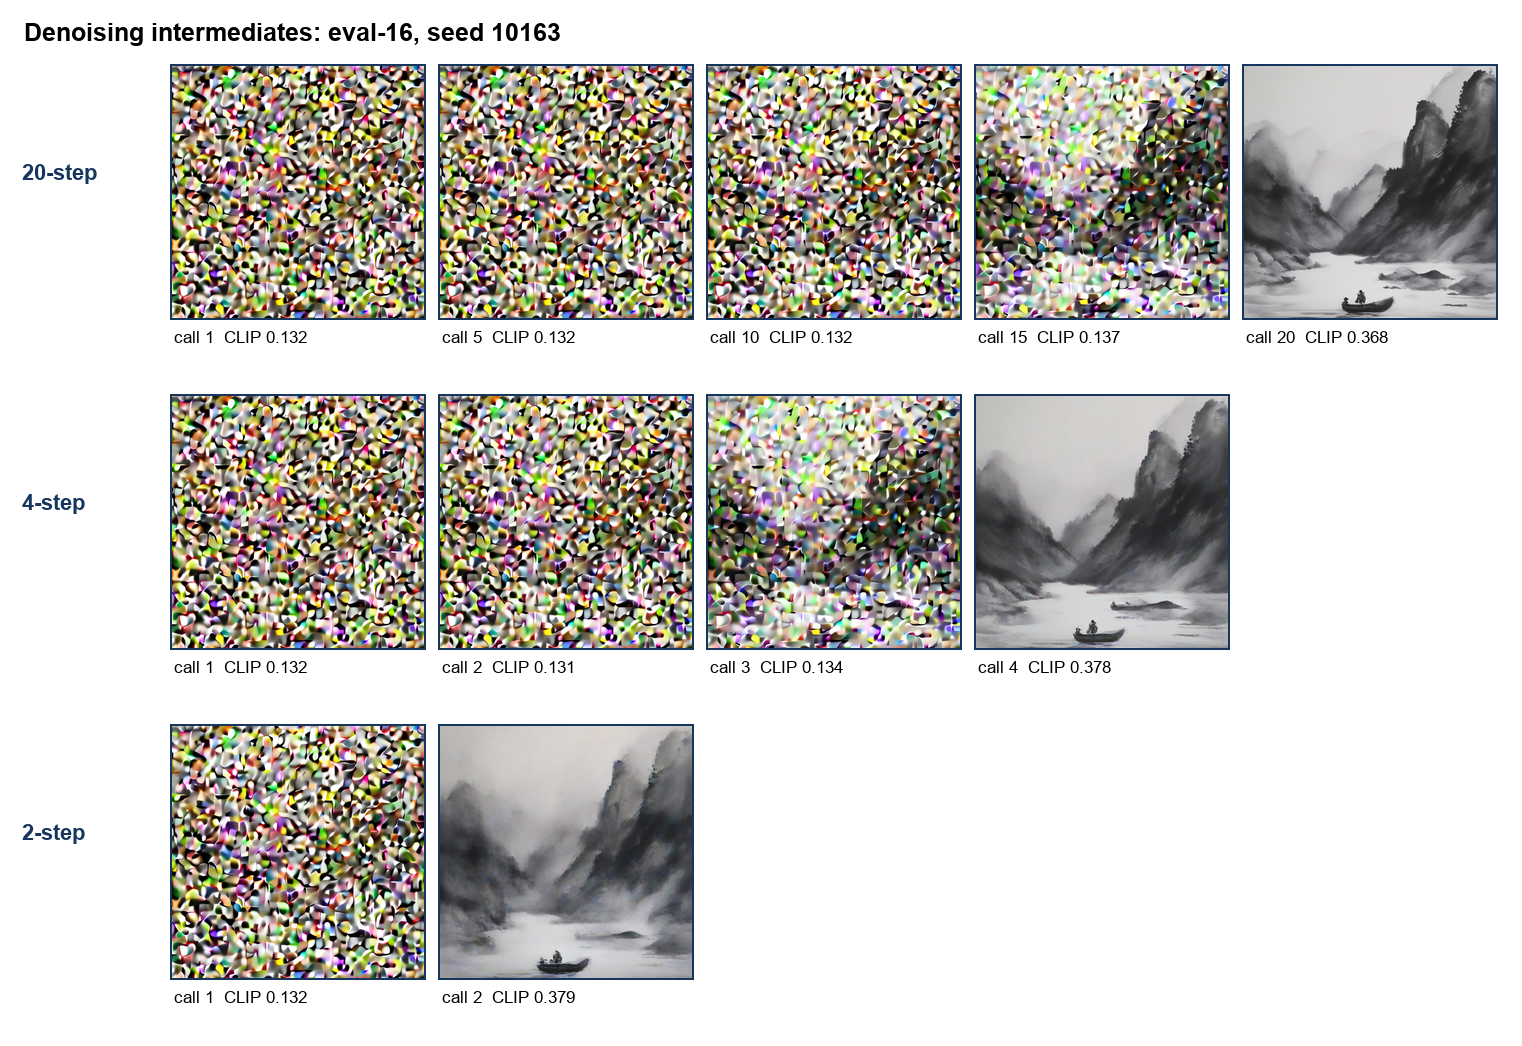
\includegraphics[width=0.96\linewidth]{figures/eval16_denoising_intermediates.png}
  \captionof{figure}{Decoded denoising states for the preferred held-out fishing-boat
  prompt at seed 10163.  Composition becomes visually measurable mainly in the
  last teacher or student transition.}
  \label{fig:intermediate-montage}
\end{center}

For reference, the teacher CLIP mean stays near 0.12 through call 14, then rises
to 0.174 (call 17), 0.234 (call 18), and $0.346\pm0.049$ (call 20).  The 4-step
sequence is 0.125, 0.122, 0.130, and $0.368\pm0.020$; the 2-step sequence is
0.122 and $0.366\pm0.014$.  These values diagnose visible emergence only:
intermediate $x_t$ is intentionally noisy and need not lie on the natural-image
manifold.  Per-call images, per-seed scores, and feature caches are retained in
the evaluation outputs for reproducibility.

\subsection{Architecture and cached representations}

\begin{table}[h]
\centering
\small
\begin{tabular}{ll}
\toprule
\textbf{Component} & \textbf{Setting} \\
\midrule
Backbone & PixArt-$\Sigma$ XL 2, 512-pixel variant \\
Full corpus & 260 image--caption pairs \\
Primary style subset & 209 plant image--caption pairs \\
Other corpus categories & 30 animal and 21 other pairs \\
Cached image features & FP16 VAE latents, $[N,4,64,64]$ \\
Cached text features & FP16 T5 embeddings, $[N,300,4096]$ \\
Teacher adapter & rank 16, alpha 16, learning rate $10^{-5}$ \\
4-step Student & four five-step phases, learning rate $5\times10^{-6}$ \\
2-step Student & two ten-step phases, learning rate $2\times10^{-6}$ \\
Trajectory cache & 627 prompts, two seeds, 1,254 trajectories \\
Student task sampling & 80\% trajectory, 20\% diffusion anchor \\
\bottomrule
\end{tabular}
\caption{Full implementation settings used by the Teacher--Student pipeline.}
\label{tab:appendix-settings}
\end{table}

\paragraph{Text conditioning and cross-attention.}
The VAE and T5 encoder are frozen and evaluated before LoRA optimization. The
VAE converts each training image into a clean latent, while T5 converts its
caption into a sequence of contextual embeddings. During Transformer training,
the noisy image-latent tokens attend to these cached text features through the
model's cross-attention blocks. The method therefore trains neither the VAE nor
the text embeddings; it updates only the attached LoRA matrices while the
frozen text features condition the denoising prediction.

\paragraph{LoRA target modules.}
The implementation is not restricted to attention weights. LoRA modules are
attached to query, key, value, and attention-output projections, together with
feed-forward and additional projection layers. Representative targets include
\texttt{ff.net.0.proj}, \texttt{ff.net.2}, \texttt{proj\_in},
\texttt{proj\_out}, \texttt{proj}, \texttt{linear}, \texttt{linear\_1}, and
\texttt{linear\_2}. The original PixArt parameters remain frozen.

\subsection{Cache validation}

All images, captions, latents, and text embeddings are linked by a deterministic
manifest. Before training, the loader checks sample identifiers, ordering,
tensor shapes, data types, finite values, and the dataset fingerprint. This
prevents a valid-looking latent from being paired silently with the wrong text
embedding. The validated cache can then be reused across LoRA ranks, learning
rates, checkpoints, and Student stages.

\section{Extended Distillation Procedure}
\label{app:distillation}

\subsection{Teacher trajectory construction}

The selected 20-step Teacher is loaded once to generate deterministic latent
trajectories. Each cached record contains 21 latent states, its prompt index,
seed, scheduler configuration, Teacher-adapter hash, and prompt-bank
fingerprint. After the cache is verified, the Teacher is removed from GPU
memory and Student optimization uses only cached trajectory states and text
conditioning.

\begin{table}[h]
\centering
\small
\begin{tabular}{lll}
\toprule
\textbf{Stage} & \textbf{Teacher-state intervals} & \textbf{Student calls} \\
\midrule
4-step Student & $(0,5),(5,10),(10,15),(15,20)$ & 4 \\
2-step Student & $(0,10),(10,20)$ & 2 \\
\bottomrule
\end{tabular}
\caption{Cached Teacher intervals learned by each Student.}
\label{tab:appendix-phases}
\end{table}

\subsection{Trajectory and anchor objectives}

For a predicted phase endpoint $\hat z_e^S$ and cached Teacher endpoint
$z_e^T$, trajectory updates use the element-wise pseudo-Huber loss
\begin{equation}
\mathcal{L}_{\mathrm{traj}}
=\operatorname{mean}\!\left(
\sqrt{(\hat z_e^S-z_e^T)^2+c^2}-c
\right),
\qquad c=10^{-3}.
\label{eq:appendix-pseudo-huber}
\end{equation}
With probability 0.8, an optimizer update uses
$\mathcal{L}_{\mathrm{traj}}$; with probability 0.2, it instead applies the
standard diffusion noise-prediction MSE to a real clean latent. Thus, 80/20 is
stochastic task sampling rather than two losses evaluated in every update.

For the second phase of the 2-step Student, half of the starting states are
generated by the current Student's first jump and detached before the second
jump. This on-policy correction exposes the model to its own first-step error
and reduces the train--test mismatch that would arise if every second-phase
input were copied from a perfect Teacher trajectory.

\subsection{Training sequence}

\begin{enumerate}
    \item Encode images with the frozen VAE and captions with the frozen T5
    encoder; validate identifiers, shapes, ordering, and hashes.
    \item Attach rank-$r$ LoRA modules to the frozen PixArt Transformer and
    train the 20-step style Teacher with diffusion MSE.
    \item Select one Teacher checkpoint using held-out prompts rather than
    assuming that the final training checkpoint is optimal.
    \item Cache deterministic 20-step Teacher trajectories for the expanded
    prompt bank and unload the Teacher.
    \item Initialize the 4-step Student from the selected Teacher LoRA and train
    it on the four intervals in Table~\ref{tab:appendix-phases}.
    \item Select an accepted 4-step checkpoint, initialize the 2-step Student
    from it, and train with two intervals and on-policy correction.
    \item Evaluate fixed checkpoints using matched prompts, seeds, schedulers,
    and exact Transformer-call counts.
\end{enumerate}

\section{Reproducibility Information}
\label{app:reproducibility}

Each reported run should record the following fields:
\begin{itemize}
    \item base-model identifier and revision;
    \item dataset, latent-cache, text-cache, and prompt-bank fingerprints;
    \item LoRA target modules, rank, alpha, learning rate, and checkpoint;
    \item scheduler class, complete timestep sequence, inference steps, and
    guidance scale;
    \item training and evaluation seeds, prompt identifiers, and sample count;
    \item Teacher and Student adapter hashes; and
    \item measured latency, hardware, precision, memory mode, and exact number
    of Transformer forward calls.
\end{itemize}
\end{document}
